\chapter{Modeling of Train Operations}
\label{chap:ModelingOfTrainOperations}
\par\noindent
\textit{\textbf{Introduction}} Chapter \ref{chap:FundamentalsOfRailwayVehicleEngineering} has established the theoretical model of the train braking process. It will serve as a foundation to build a practical model suitable for conducting actual simulations. 

\section{Matlab Simulink}
\label{sec:MatlabSimulink}
The model has been built utilizing the software Matlab Simulink by Mathworks. It offers several distinct advantages: It uses a graphical block diagramming tool which makes it very intuitive to use. At the same time, various official and third-party add-on libraries make it very versatile. Most importantly, as it is tightly integrated with the Matlab environment, it can be used for both modeling and simulating dynamical systems, like the braking process of a train.

\section{Initial Model}
\label{sec:InitialModel}
\par\noindent
Looking back at chapter \ref{chap:FundamentalsOfRailwayVehicleEngineering}, the aim is to build a model for the braking process of a freight train. An initial model of a single braking procedure, kindly provided by Dr. Raphael Pfaff, will serve as a basis. Most of the components previously designed in chapter \ref{chap:FundamentalsOfRailwayVehicleEngineering} can already be found therein.  

\begin{figure}[H]
	\centering
	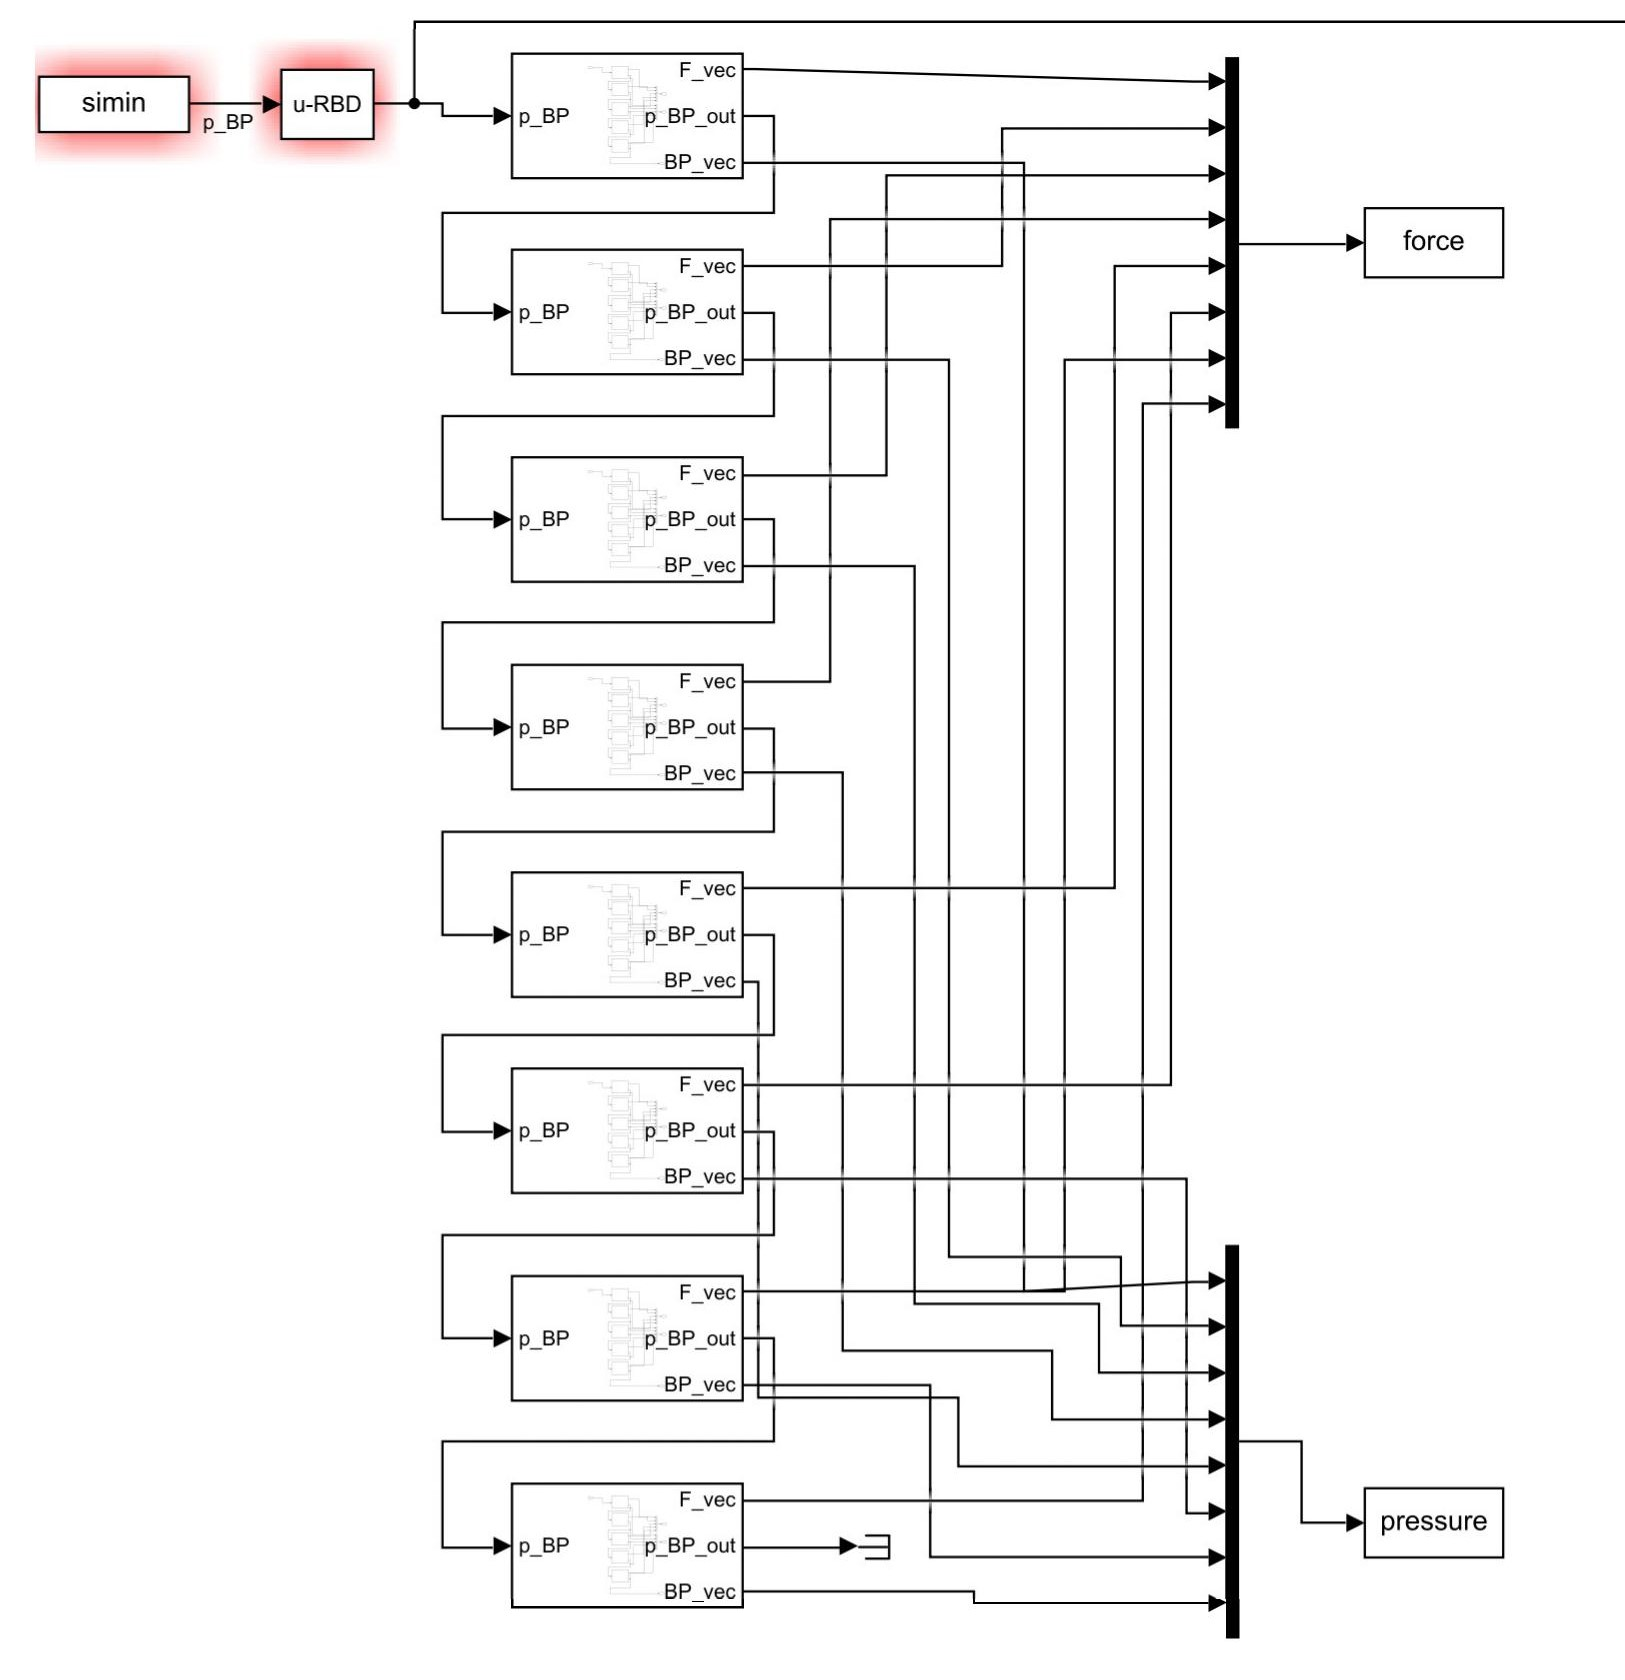
\includegraphics[width=\linewidth]{./pic/initmodel_whole}
	\caption{Initial Model}
	\label{fig:initmodel_whole}
\end{figure}

\par\noindent
Figure \ref{fig:initmodel_whole} shows a model of a freight train of fixed length, consisting of 40 wagons in total. For better readability, five wagons are condensed into one subsystem each, marked by the red rectangle. The subsystems are interconnected by a brake pipe, marked by the green arrow. They have one input port for the incoming pressure on the brake pipe, and three output ports, one for the pipe connection to the next subsystem, and two for recording brake pressure and brake force (marked by the pink and blue arrows, respectively). A depiction of a subsystem can be found in appendix \ref{fig:initmodel_subsys}.  

\begin{figure}[H]
	\centering
	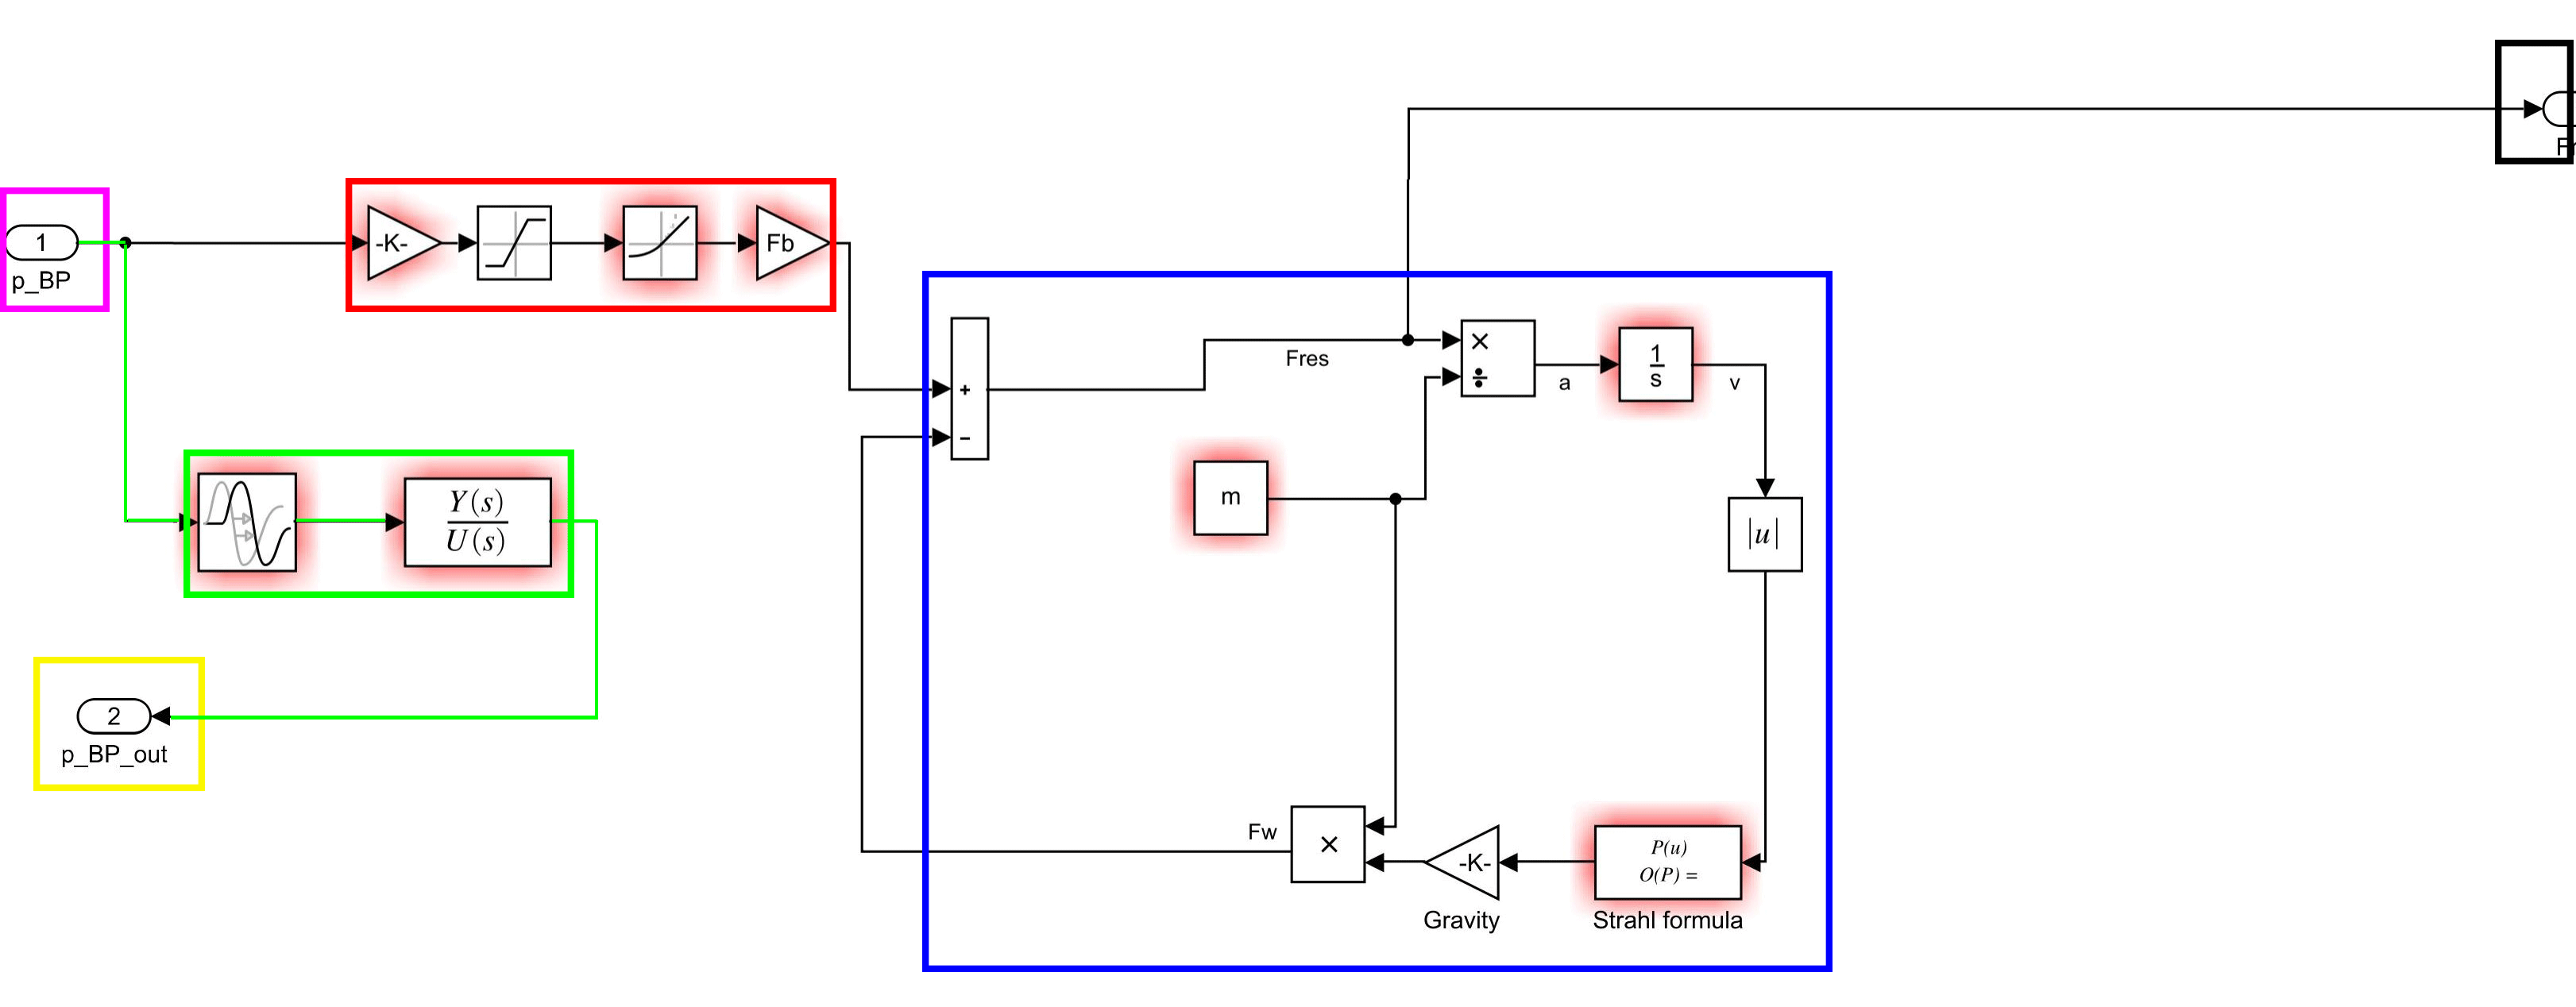
\includegraphics[width=\linewidth]{./pic/initmodel_wagon}
	\caption{Initial Model - Wagon}
	\label{fig:initmodel_wagon}
\end{figure}

\par\noindent
Figure \ref{fig:expandedmodel_wagon} shows a model of a freight wagon. It already encompasses several of the model variables defined in section \ref{sec:InherentFactors}. The brake pipe ${\mathcal{M}}_{bp}$ is represented by the green arrows. It leads from input port (pink rectangle) to output port (yellow rectangle); the propagation delay is realized by a transport delay block (green rectangle), using propagation velocity $v_{bp}$ and wagon length $l_{bp}$. The brake pressure $p_{bp}$ is the value of the signal traveling through the connection. Note that in the simulation, the signal value for $p_{bp}$ is the difference between regular operating pressure and actual pressure, e.g. if simulated pressure on the brake pipe is 3.5 bar, the signal value is $3.5 - 5 = -1.5$.
\par
The brake cylinder ${\mathcal{M}}_{bc}$ is represented by the red rectangle. The pressure on the brake pipe $p_{bp}$ is converted into a coefficient between zero and one, where zero equals no brakes applied, or $p_{bp} = 5$, and one equals full braking pressure, or $p_{bp} = 3.5$. The exact formula is this:

\begin{align*}
p_{bc} = p_{bp} \cdot \frac{-1}{5-3.5}
\end{align*}

\noindent
So for a braking pressure of 4 bar, the coefficient would be $(4 - 5) \cdot \frac{-1}{5-3.5} = -1 \cdot \frac{-1}{1.5} = \frac{2}{3}$. A rate limiter block accounts for the brake cylinder's filling time $t_{bc}$. Finally, the braking force is calculated by multiplying the maximum braking force, which is mainly dependent on the wagon mass $m$ [train braking, 22]. So for the braking pressure, we have:

\begin{align*}
F_{b} = F_{b,max} \cdot p_{bc}
\end{align*}

\noindent
The final component is the factoring in of the driving resistance of the train, utilizing Strahl's formula. This is represented by the blue rectangle. By continuous-time integration of the acceleration, which is calculated according to Newton's second law of motion ($a = \frac{F}{m})$, it is possible to determine the velocity, which in turn allows for the calculation of the force generated by the driving resistance, This force is then added to the braking force and fed into an output port, marked with the black rectangle.
\par
Regarding simulation, this initial model is only fit for one single braking process, where a train of fixed length and fixed composition, brakes from an initial velocity all the way to a halt; the only variation is the pressure on the brake pipe, which is also the sole input for the simulation. Appendix \ref{fig:initmodel_input} shows how that input might look like.

\section{Model Expansion}
\label{sec:ModelExpansion}

\par\noindent
This initial model is however not of sufficient detail. Where it merely describes one single braking process, we need to simulate a whole ride, with alternating phases of braking and accelerating. For that purpose, the simulation input has to be adjusted accordingly. Where previously it was only one braking process, using braking pressure as input was the obvious choice, whereas now the idea is to use a kind of track profile, which shall describe the maximum allowed velocity over time, of a notional track. For visualization, please refer to \ref{fig:expandedmodel_siminput}. The simulation then only needs to brake or accelerate depending on train velocity versus maximum velocity at the current time.

\par
Accordingly, the first expansion step is to create a mechanism to control the train so to speak. For this purpose, the system simply checks for each timestamp whether the current velocity of the train is greater than the maximum allowed velocity at the current time, according to simulation input. If this is the case, a braking pressure is applied to the pipe, scaling with the difference between $v_{max}$ and $v_{real}$, $v_{dif}$. This means the higher $v_{dif}$ is, the more braking pressure gets applied. This more or less covers the braking part of the system.

\par
The model however also needs a component for acceleration. To simplify things, the logic here is that if the train is not braking, it is accelerating, which actually works out pretty well. To accelerate, a traction force is applied, which also scales with $v_{dif}$, so the higher $v_{dif}$, the higher the applied traction force.

\begin{figure}[H]
	\centering
	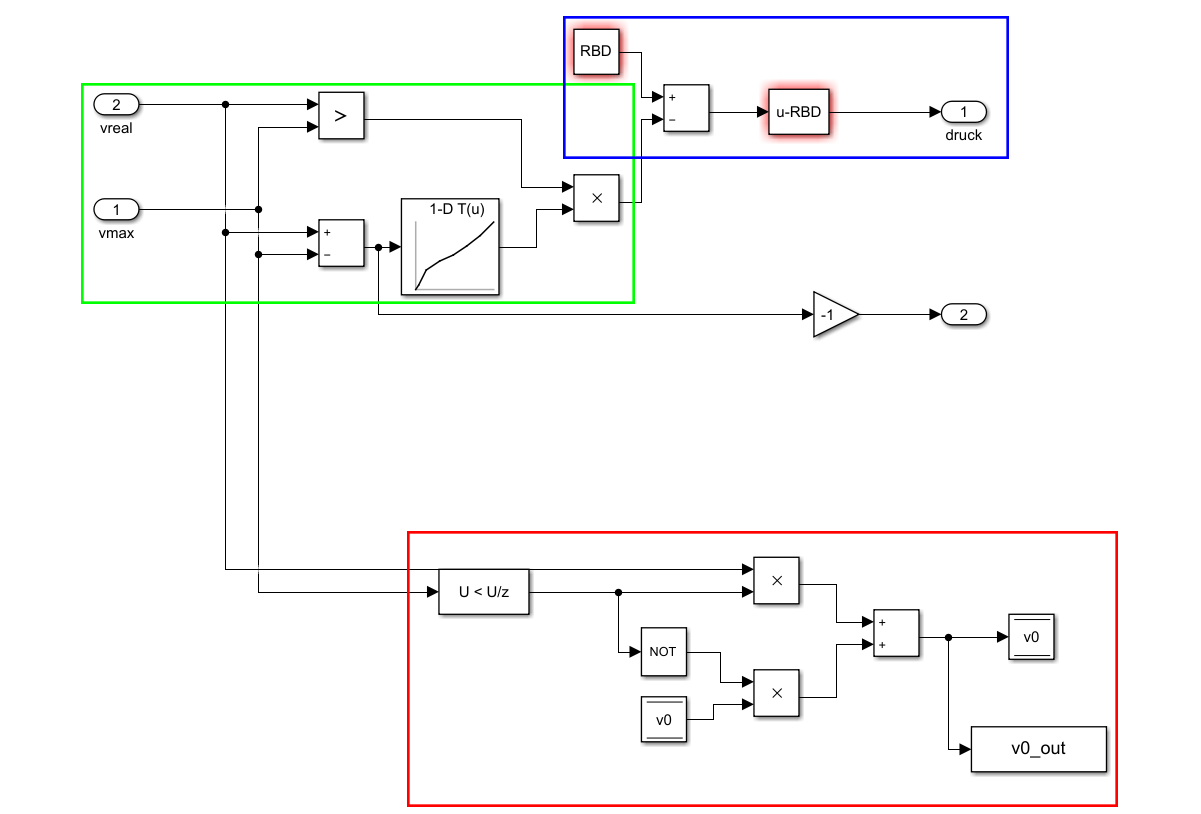
\includegraphics[width=\linewidth]{./pic/expandedmodel_pressure}
	\caption{Expanded Model - Pressure Calculation}
	\label{fig:expandedmodel_pressure}
\end{figure}

\par\noindent
Depicted above is the system which determines braking pressure to apply. It calculates $v_{dif}$ by subtracting $v_{max}$ from $v_{real}$, which is then fed into a one-dimensional lookup table. The table is a sampled representation of a function with fixed breakpoints, mapping one function value to each breakpoint, like so

\begin{equation}
\label{eq:lookuptable}
H(n) =
\begin{cases}
0.1 & \text{if $n=1$} \\
0.7 & \text{if $n=15$} \\
0.8 & \text{if $n=20$} \\
\text{..}
\end{cases}
\end{equation}

\noindent
where $n$ is the breakpoints of $v_{dif}$. Since the pressure should only be applied if $v_{real}$ is greater than $v_{max}$, the ultimate result follows the logic of the following equation

\begin{equation}
\label{eq:brakingpressure}
P(n,t) = H(n) * (v_{real}(t) > v_{max}(t))
\end{equation}

\noindent
where $v_{real}(t)$ is train velocity over time, $v_{max}(t)$ is maximum velocity over time, and $v_{real}(t) > v_{max}(t)$ is either 1 or 0.

\begin{figure}[H]
	\centering
	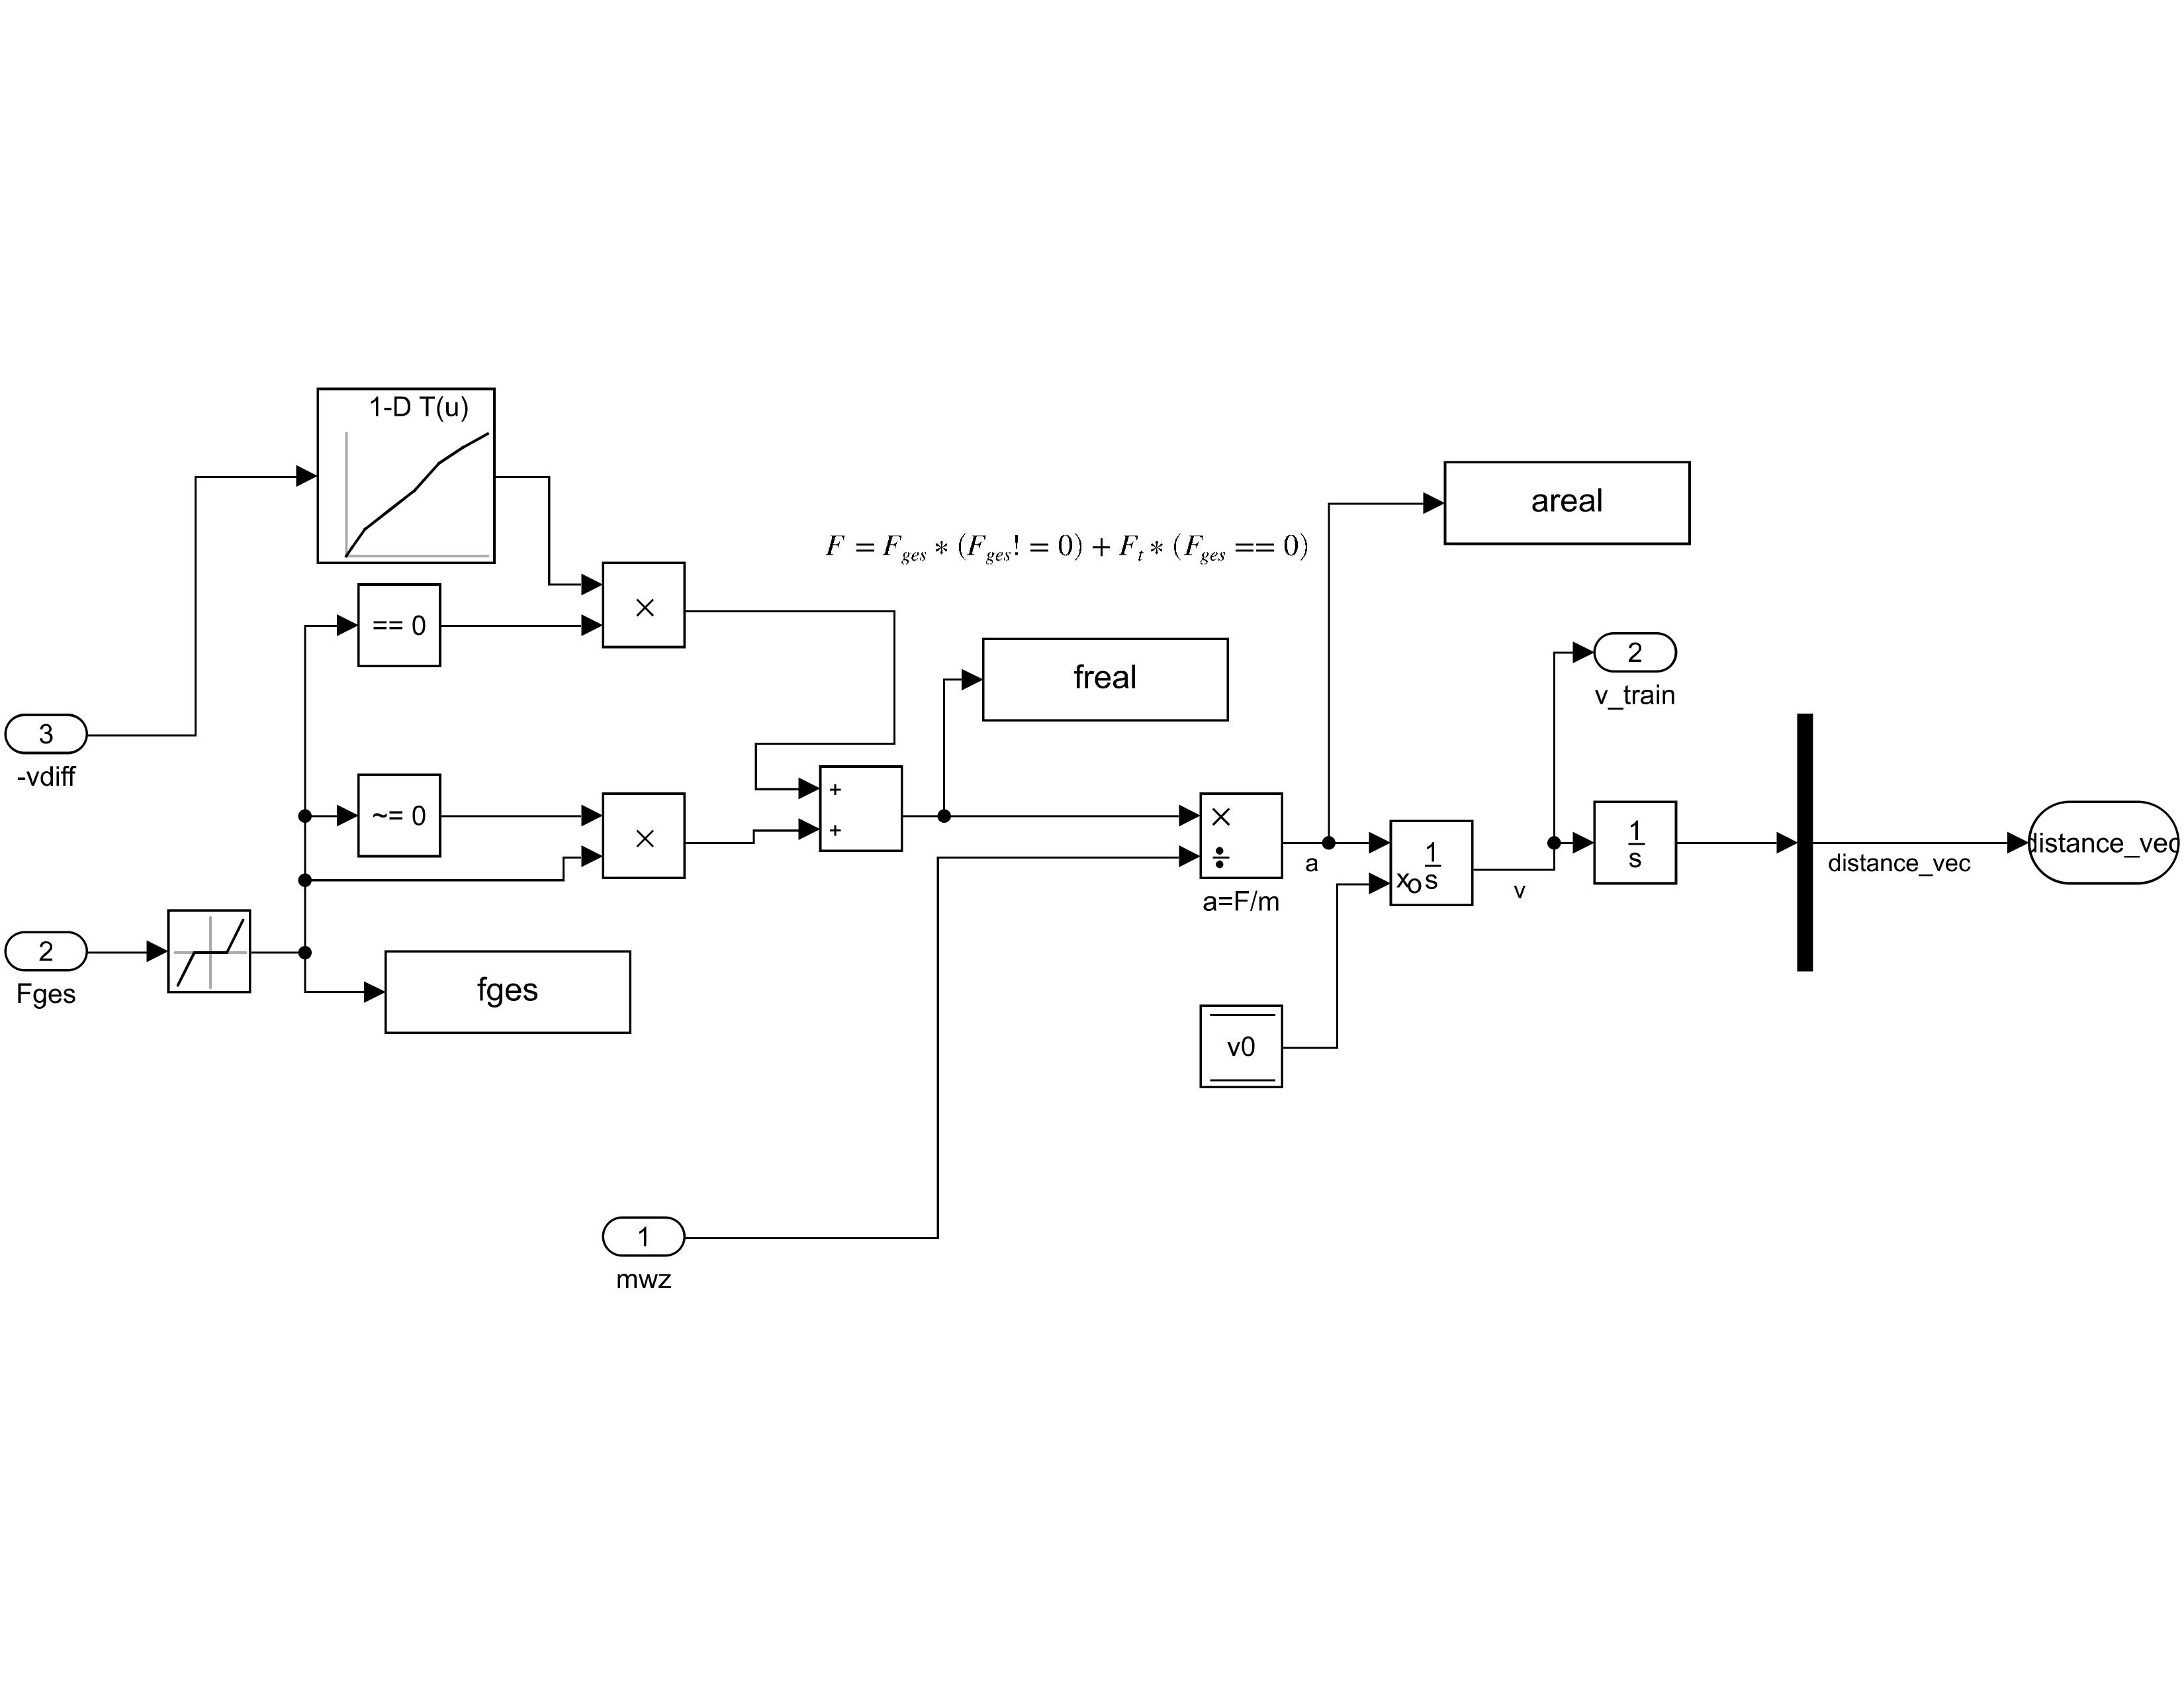
\includegraphics[width=\linewidth]{./pic/expandedmodel_force}
	\caption{Expanded Model - Traction Force Calculation}
	\label{fig:expandedmodel_force}
\end{figure}

\par\noindent
The above system determines the traction force to apply. As has been discussed earlier, this works like a simple bang-bang controller. The design is very similar to the braking pressure system: $v_{dif}$ is again fed into a one-dimensional lookup table, which outputs different values for traction force accordingly. The higher $v_{dif}$ is, the higher the traction force to apply. It is then added to the current braking force, however only either traction or braking force is at any given time positive while the other is zero, which is achieved by the equations
 
\begin{equation}
\label{eq:tracforce}
f(n,t) = H(n) * (F_{B}(t) == 0) 
\end{equation}

\noindent
where $n$ is $v_{dif}$, $H(n)$ is the lookup table function (see equation \ref{eq:lookuptable}), $F_{B}(t)$ is the braking force over time, and 

\begin{equation}
\label{eq:brakeforce}
g(t) = F_{B}(t) * (F_{B}(t) \neq 0)
\end{equation}

\noindent
where $F_{B}(t)$ is the braking force over time, so we have 

\begin{equation}
\label{eq:force}
F(n,t) = f(n,t) + g(t) 
\end{equation} 

\noindent
where $F$ is the actual force over time, either braking or traction.

\par\noindent
$F$ is then used to calculate acceleration. According to Newton's Second Law,
\begin{equation}
\label{eq:newton}
F = m * a
\end{equation}
Accordingly, acceleration is
\begin{equation}
\label{eq:acceleration}
a = F(n,t) / m
\end{equation}
	
\noindent
where $m$ is the accumulated mass of all wagons and $F(n,t)$ relates to equation \ref{eq:force}. The acceleration is then used to calculate the velocity by integrating $a$ in relation to $v_{0}$, which is the initial velocity of the current braking or acceleration process \TODO{überprüfen..}. Integration of $v$ in turn allows calculation of the traveled distance.

\begin{figure}[H]
	\centering
	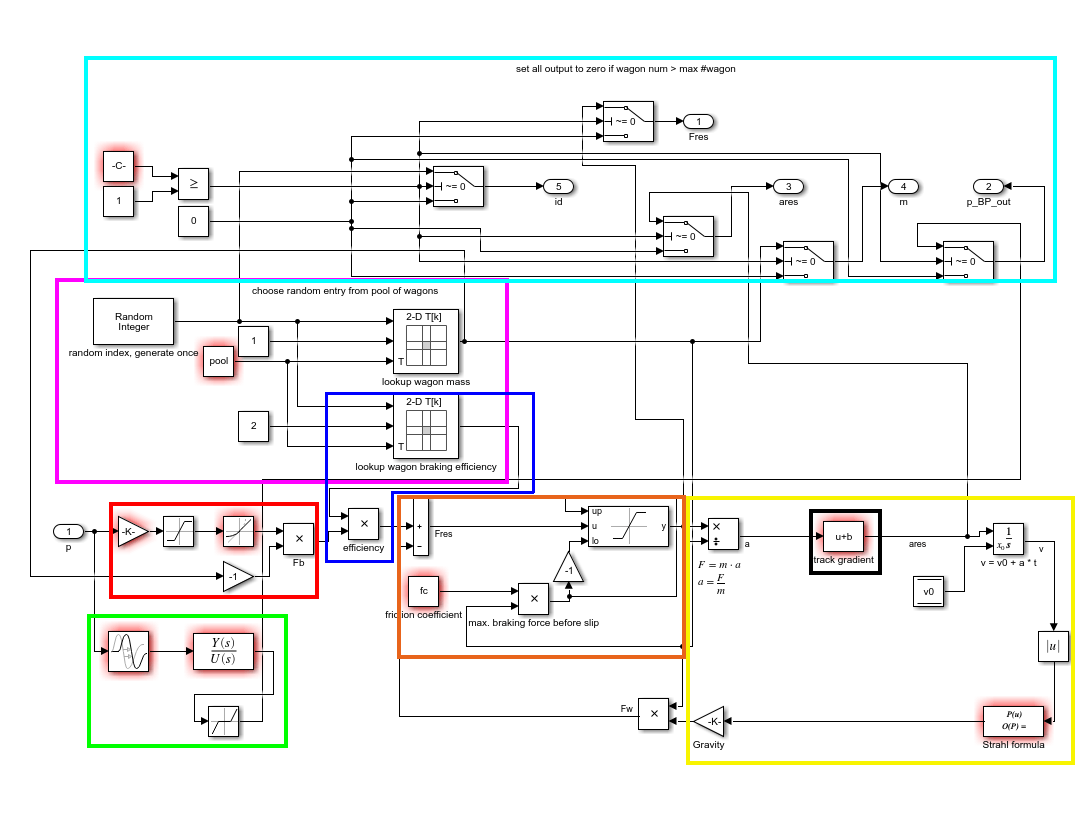
\includegraphics[width=\linewidth]{./pic/expandedmodel_wagon}
	\caption{Expanded Model - Wagon}
	\label{fig:expandedmodel_wagon}
\end{figure}

\par\noindent
The last subsystem is the actual wagon. We will take a look at the largely unchanged elements first. The sole input is still the braking pressure on the brake pipe. Simulation of the propagation delay has also remained the same as before. 

\par
One new addition is a pool of different wagons. Whereas before all 40 were distinguishable only by their position, they are now assigned with different parameters. To that end, a pool of 500 wagons has been randomly generated via python script, where each wagon has a unique ID, as well as randomly generated mass and braking efficiency. In actual simulation, up to 40 of these 500 are, currently by generation of random indices, selected and their properties used accordingly. It would also be possible to determine the wagon ids to be used beforehand, instead of choosing randomly.

\par
Another requirement was to make the number of wagons variable. In the initial model, the modeled train had a fixed number of 40 wagons, therefore also 40 wagon subsystems. Unfortunately, simulink offers no way to disable certain subsystems dynamically, but only by manually turning them off via model explorer, which would be unfeasible for such a large number of simulations. To circumvent this issue, output gets disabled for all unwanted wagons. For a simulation of a train of 20 wagons, the first 20 remain untouched, while the latter 20 produce no output and therefore also have no impact on the overall simulation. The turning off is achieved by simple switches; each wagon subsystem has a unique index from one to forty. If the index is greater than the specified number of wagons, all switches are turned to output zero.
	
\section{Further Expansion}
\label{sec:FurtherExpansion}